\documentclass[tikz,border=0pt]{standalone}
\usepackage{xcolor}
\usetikzlibrary{calc}
% Palette: Sam_Comm_final.png by eye, and the drones and raiders.
\definecolor{ink}{HTML}{3B2340}
\definecolor{sky}{HTML}{EFC46A}
\definecolor{skyhi}{HTML}{F5DA92}
\definecolor{skylow}{HTML}{E9B060}
\definecolor{cloud}{HTML}{F2D58A}
\definecolor{paper}{HTML}{FBEFD0}
\definecolor{cream}{HTML}{FFF6E0}
\definecolor{white}{HTML}{FFFFFF}
\definecolor{wallA}{HTML}{E88A73}
\definecolor{wallB}{HTML}{EE9F7E}
\definecolor{wallC}{HTML}{E47A7E}
\definecolor{wallD}{HTML}{F0B07E}
\definecolor{wallE}{HTML}{D9765F}
\definecolor{wallF}{HTML}{E99A8A}
\definecolor{greenA}{HTML}{8DBB7E}
\definecolor{greenB}{HTML}{6FA77A}
\definecolor{greenC}{HTML}{A9C97F}
\definecolor{greenD}{HTML}{5E9C6A}
\definecolor{greenE}{HTML}{4A8060}
\definecolor{sage}{HTML}{9DB98A}
\definecolor{sagedark}{HTML}{6F8F66}
\definecolor{sagelight}{HTML}{C2D6A6}
\definecolor{window}{HTML}{F6E7A0}
\definecolor{windark}{HTML}{8C5A64}
\definecolor{metal}{HTML}{8D9A93}
\definecolor{metaldark}{HTML}{5E6B66}
\definecolor{metallight}{HTML}{B9C4BC}
\definecolor{wood}{HTML}{B9835A}
\definecolor{wooddark}{HTML}{8C5A3C}
\definecolor{woodlight}{HTML}{D9A66F}
\definecolor{stone}{HTML}{E7C9A0}
\definecolor{stonedark}{HTML}{C9A47E}
\definecolor{concrete}{HTML}{D8C3A4}
\definecolor{concretedark}{HTML}{B8A084}
\definecolor{asphalt}{HTML}{8E7A86}
\definecolor{asphaltdark}{HTML}{6E5C68}
\definecolor{roadline}{HTML}{F6E7A0}
\definecolor{kerb}{HTML}{D8B48C}
\definecolor{red}{HTML}{E0483E}
\definecolor{redlight}{HTML}{F27A6A}
\definecolor{gold}{HTML}{FFB000}
\definecolor{goldlight}{HTML}{FFD54F}
\definecolor{teal}{HTML}{4FA3A0}
\definecolor{tealdark}{HTML}{3C8582}
\definecolor{magenta}{HTML}{FF2E88}
\definecolor{cyan}{HTML}{13CFE3}
\definecolor{violet}{HTML}{8A5BD6}
\definecolor{orange}{HTML}{F2803A}
\definecolor{pink}{HTML}{F48FB1}
\definecolor{glow}{HTML}{4FE6E0}
\definecolor{glowhi}{HTML}{C8FFF9}
\definecolor{hot}{HTML}{FF6A1A}
\definecolor{hothi}{HTML}{FFD07A}
\definecolor{armour}{HTML}{7E7A86}
\definecolor{armourdark}{HTML}{5A5466}
\definecolor{armourlight}{HTML}{A8A2B0}
\definecolor{wasp}{HTML}{E0A82E}
\definecolor{waspdark}{HTML}{B07E1A}
\definecolor{moth}{HTML}{F2E6C8}
\definecolor{mothdark}{HTML}{D2C09A}
\definecolor{hornet}{HTML}{3C8582}
\definecolor{hornetdark}{HTML}{2C6260}
\definecolor{warden}{HTML}{E47A7E}
\definecolor{wardendark}{HTML}{B85A62}
\definecolor{tick}{HTML}{8DBB7E}
\definecolor{tickdark}{HTML}{5E8A5A}
\definecolor{strider}{HTML}{D9765F}
\definecolor{striderdark}{HTML}{A8543F}
\definecolor{jacket}{HTML}{6FA77A}
\definecolor{jacketb}{HTML}{4FA3A0}
\definecolor{jacketc}{HTML}{E88A73}
\definecolor{jacketd}{HTML}{F0B07E}
\definecolor{skin}{HTML}{F2C49A}
\definecolor{skinb}{HTML}{C98C6A}
\definecolor{skinc}{HTML}{8C5A3C}
\definecolor{hair}{HTML}{3B2340}
\definecolor{goo}{HTML}{B6E35A}
\definecolor{goodark}{HTML}{7FB23A}
\newcommand{\Ink}{1.15pt}
\tikzset{inked/.style={draw=ink, line width=\Ink, line join=round, line cap=round}}
\begin{document}
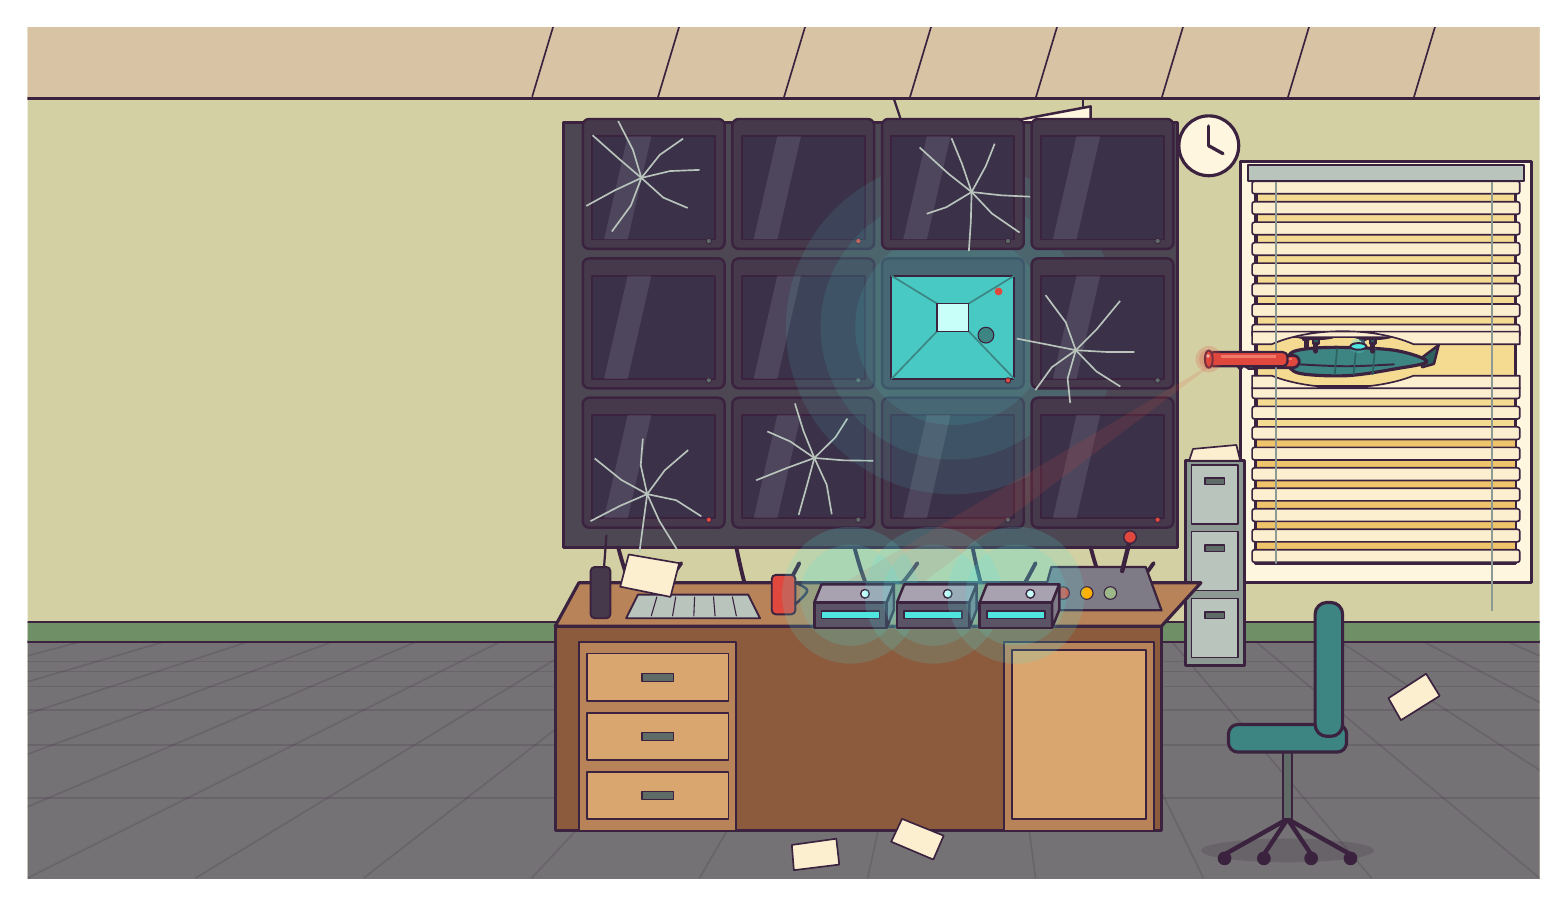
\begin{tikzpicture}
\clip (0,0) rectangle (19.2,10.8);
\filldraw[inked,fill=sagelight!55!stone] (-0.5,-0.5) rectangle (19.7,11.3);
\filldraw[inked,fill=concrete] (-0.5,9.9) rectangle (19.7,11.3);
\draw[ink, line width=1pt, line cap=round] (-0.5,9.9) -- (19.7,9.9);
\filldraw[inked,fill=metaldark!55!asphalt] (-0.5,-0.5) rectangle (19.7,3);
\filldraw[inked,fill=sagedark,line width=0.9pt] (-0.5,3) rectangle (19.7,3.25);
\draw[ink, opacity=0.18, line width=0.6pt] (-19.2,0) -- (-3.6,3);
\draw[ink, opacity=0.18, line width=0.6pt] (-17.067,0) -- (-2.533,3);
\draw[ink, opacity=0.18, line width=0.6pt] (-14.933,0) -- (-1.467,3);
\draw[ink, opacity=0.18, line width=0.6pt] (-12.8,0) -- (-0.4,3);
\draw[ink, opacity=0.18, line width=0.6pt] (-10.667,0) -- (0.667,3);
\draw[ink, opacity=0.18, line width=0.6pt] (-8.533,0) -- (1.733,3);
\draw[ink, opacity=0.18, line width=0.6pt] (-6.4,0) -- (2.8,3);
\draw[ink, opacity=0.18, line width=0.6pt] (-4.267,0) -- (3.867,3);
\draw[ink, opacity=0.18, line width=0.6pt] (-2.133,0) -- (4.933,3);
\draw[ink, opacity=0.18, line width=0.6pt] (0,0) -- (6,3);
\draw[ink, opacity=0.18, line width=0.6pt] (2.133,0) -- (7.067,3);
\draw[ink, opacity=0.18, line width=0.6pt] (4.267,0) -- (8.133,3);
\draw[ink, opacity=0.18, line width=0.6pt] (6.4,0) -- (9.2,3);
\draw[ink, opacity=0.18, line width=0.6pt] (8.533,0) -- (10.267,3);
\draw[ink, opacity=0.18, line width=0.6pt] (10.667,0) -- (11.333,3);
\draw[ink, opacity=0.18, line width=0.6pt] (12.8,0) -- (12.4,3);
\draw[ink, opacity=0.18, line width=0.6pt] (14.933,0) -- (13.467,3);
\draw[ink, opacity=0.18, line width=0.6pt] (17.067,0) -- (14.533,3);
\draw[ink, opacity=0.18, line width=0.6pt] (19.2,0) -- (15.6,3);
\draw[ink, opacity=0.18, line width=0.6pt] (21.333,0) -- (16.667,3);
\draw[ink, opacity=0.18, line width=0.6pt] (23.467,0) -- (17.733,3);
\draw[ink, opacity=0.18, line width=0.6pt] (25.6,0) -- (18.8,3);
\draw[ink, opacity=0.18, line width=0.6pt] (27.733,0) -- (19.867,3);
\draw[ink, opacity=0.18, line width=0.6pt] (29.867,0) -- (20.933,3);
\draw[ink, opacity=0.18, line width=0.6pt] (32,0) -- (22,3);
\draw[ink, opacity=0.18, line width=0.6pt] (34.133,0) -- (23.067,3);
\draw[ink, opacity=0.18, line width=0.6pt] (36.267,0) -- (24.133,3);
\draw[ink, opacity=0.18, line width=0.6pt] (38.4,0) -- (25.2,3);
\draw[ink, opacity=0.18, line width=0.6pt] (-1,1.02) -- (20.2,1.02);
\draw[ink, opacity=0.18, line width=0.6pt] (-1,1.693) -- (20.2,1.693);
\draw[ink, opacity=0.18, line width=0.6pt] (-1,2.138) -- (20.2,2.138);
\draw[ink, opacity=0.18, line width=0.6pt] (-1,2.431) -- (20.2,2.431);
\draw[ink, opacity=0.18, line width=0.6pt] (-1,2.624) -- (20.2,2.624);
\draw[ink, opacity=0.18, line width=0.6pt] (-1,2.752) -- (20.2,2.752);
\begin{scope}\clip (6.4,-1) rectangle (20.2,11.8);
\draw[ink, line width=0.6pt, line cap=round] (6.4,9.9) -- (6.7,10.9);
\draw[ink, line width=0.6pt, line cap=round] (8,9.9) -- (8.3,10.9);
\draw[ink, line width=0.6pt, line cap=round] (9.6,9.9) -- (9.9,10.9);
\draw[ink, line width=0.6pt, line cap=round] (11.2,9.9) -- (11.5,10.9);
\draw[ink, line width=0.6pt, line cap=round] (12.8,9.9) -- (13.1,10.9);
\draw[ink, line width=0.6pt, line cap=round] (14.4,9.9) -- (14.7,10.9);
\draw[ink, line width=0.6pt, line cap=round] (16,9.9) -- (16.3,10.9);
\draw[ink, line width=0.6pt, line cap=round] (17.6,9.9) -- (17.9,10.9);
\draw[ink, line width=0.6pt, line cap=round] (19.2,9.9) -- (19.5,10.9);
\draw[ink, line width=0.8pt, line cap=round] (11,9.9) -- (11.2,9.3);
\draw[ink, line width=0.8pt, line cap=round] (13.4,9.9) -- (13.4,9.75);
\filldraw[inked,fill=cream,line width=0.9pt] (11.1,9.35) -- (13.5,9.8) -- (13.5,9.6) -- (11.1,9.15) -- cycle;
\filldraw[inked,fill=ink!50!metaldark] (6.8,4.2) rectangle (14.6,9.6);
\filldraw[inked,fill=ink!70!metaldark,rounded corners=0.08cm,line width=0.9pt] (7.05,4.45) rectangle (8.85,6.1);
\filldraw[inked,fill=ink!85!tealdark,line width=0.7pt] (7.17,4.57) rectangle (8.73,5.88);
\fill[white, opacity=0.1] (7.32,4.57) -- (7.62,4.57) -- (7.92,5.88) -- (7.62,5.88) -- cycle;
\draw[metallight, line width=0.6pt, line join=round] (7.868,4.876) -- (8.235,4.799) -- (8.555,4.594);
\draw[metallight, line width=0.6pt, line join=round] (7.868,4.876) -- (8.09,5.178) -- (8.388,5.435);
\draw[metallight, line width=0.6pt, line join=round] (7.868,4.876) -- (7.786,5.242) -- (7.812,5.581);
\draw[metallight, line width=0.6pt, line join=round] (7.868,4.876) -- (7.539,5.057) -- (7.201,5.329);
\draw[metallight, line width=0.6pt, line join=round] (7.868,4.876) -- (7.523,4.727) -- (7.148,4.533);
\draw[metallight, line width=0.6pt, line join=round] (7.868,4.876) -- (7.818,4.504) -- (7.77,4.142);
\draw[metallight, line width=0.6pt, line join=round] (7.868,4.876) -- (8.023,4.534) -- (8.246,4.173);
\filldraw[inked,fill=red,line width=0.3pt] (8.65,4.55) circle (0.035);
\filldraw[inked,fill=ink!70!metaldark,rounded corners=0.08cm,line width=0.9pt] (7.05,6.22) rectangle (8.85,7.87);
\filldraw[inked,fill=ink!85!tealdark,line width=0.7pt] (7.17,6.34) rectangle (8.73,7.65);
\fill[white, opacity=0.1] (7.32,6.34) -- (7.62,6.34) -- (7.92,7.65) -- (7.62,7.65) -- cycle;
\filldraw[inked,fill=metaldark,line width=0.3pt] (8.65,6.32) circle (0.035);
\filldraw[inked,fill=ink!70!metaldark,rounded corners=0.08cm,line width=0.9pt] (7.05,7.99) rectangle (8.85,9.64);
\filldraw[inked,fill=ink!85!tealdark,line width=0.7pt] (7.17,8.11) rectangle (8.73,9.42);
\fill[white, opacity=0.1] (7.32,8.11) -- (7.62,8.11) -- (7.92,9.42) -- (7.62,9.42) -- cycle;
\draw[metallight, line width=0.6pt, line join=round] (7.794,8.892) -- (8.159,8.979) -- (8.533,8.994);
\draw[metallight, line width=0.6pt, line join=round] (7.794,8.892) -- (8.028,9.185) -- (8.323,9.39);
\draw[metallight, line width=0.6pt, line join=round] (7.794,8.892) -- (7.686,9.251) -- (7.5,9.613);
\draw[metallight, line width=0.6pt, line join=round] (7.794,8.892) -- (7.509,9.135) -- (7.174,9.433);
\draw[metallight, line width=0.6pt, line join=round] (7.794,8.892) -- (7.454,8.733) -- (7.094,8.536);
\draw[metallight, line width=0.6pt, line join=round] (7.794,8.892) -- (7.661,8.541) -- (7.419,8.211);
\draw[metallight, line width=0.6pt, line join=round] (7.794,8.892) -- (8.073,8.641) -- (8.382,8.51);
\filldraw[inked,fill=metaldark,line width=0.3pt] (8.65,8.09) circle (0.035);
\filldraw[inked,fill=ink!70!metaldark,rounded corners=0.08cm,line width=0.9pt] (8.95,4.45) rectangle (10.75,6.1);
\filldraw[inked,fill=ink!85!tealdark,line width=0.7pt] (9.07,4.57) rectangle (10.63,5.88);
\fill[white, opacity=0.1] (9.22,4.57) -- (9.52,4.57) -- (9.82,5.88) -- (9.52,5.88) -- cycle;
\draw[metallight, line width=0.6pt, line join=round] (9.991,5.335) -- (10.365,5.305) -- (10.74,5.3);
\draw[metallight, line width=0.6pt, line join=round] (9.991,5.335) -- (10.259,5.598) -- (10.41,5.835);
\draw[metallight, line width=0.6pt, line join=round] (9.991,5.335) -- (9.851,5.682) -- (9.744,6.027);
\draw[metallight, line width=0.6pt, line join=round] (9.991,5.335) -- (9.682,5.546) -- (9.394,5.672);
\draw[metallight, line width=0.6pt, line join=round] (9.991,5.335) -- (9.639,5.207) -- (9.252,5.052);
\draw[metallight, line width=0.6pt, line join=round] (9.991,5.335) -- (9.893,4.973) -- (9.792,4.613);
\draw[metallight, line width=0.6pt, line join=round] (9.991,5.335) -- (10.148,4.994) -- (10.212,4.62);
\filldraw[inked,fill=metaldark,line width=0.3pt] (10.55,4.55) circle (0.035);
\filldraw[inked,fill=ink!70!metaldark,rounded corners=0.08cm,line width=0.9pt] (8.95,6.22) rectangle (10.75,7.87);
\filldraw[inked,fill=ink!85!tealdark,line width=0.7pt] (9.07,6.34) rectangle (10.63,7.65);
\fill[white, opacity=0.1] (9.22,6.34) -- (9.52,6.34) -- (9.82,7.65) -- (9.52,7.65) -- cycle;
\filldraw[inked,fill=metaldark,line width=0.3pt] (10.55,6.32) circle (0.035);
\filldraw[inked,fill=ink!70!metaldark,rounded corners=0.08cm,line width=0.9pt] (8.95,7.99) rectangle (10.75,9.64);
\filldraw[inked,fill=ink!85!tealdark,line width=0.7pt] (9.07,8.11) rectangle (10.63,9.42);
\fill[white, opacity=0.1] (9.22,8.11) -- (9.52,8.11) -- (9.82,9.42) -- (9.52,9.42) -- cycle;
\filldraw[inked,fill=red,line width=0.3pt] (10.55,8.09) circle (0.035);
\filldraw[inked,fill=ink!70!metaldark,rounded corners=0.08cm,line width=0.9pt] (10.85,4.45) rectangle (12.65,6.1);
\filldraw[inked,fill=ink!85!tealdark,line width=0.7pt] (10.97,4.57) rectangle (12.53,5.88);
\fill[white, opacity=0.1] (11.12,4.57) -- (11.42,4.57) -- (11.72,5.88) -- (11.42,5.88) -- cycle;
\filldraw[inked,fill=metaldark,line width=0.3pt] (12.45,4.55) circle (0.035);
\filldraw[inked,fill=ink!70!metaldark,rounded corners=0.08cm,line width=0.9pt] (10.85,6.22) rectangle (12.65,7.87);
\fill[glow, opacity=0.1] (11.75,6.995) circle (2.12);
\fill[glow, opacity=0.1] (11.75,6.995) circle (1.68);
\fill[glow, opacity=0.1] (11.75,6.995) circle (1.24);
\filldraw[inked,fill=glow!70!tealdark,line width=0.7pt] (10.97,6.34) rectangle (12.53,7.65);
\draw[tealdark, line width=0.6pt, line cap=round] (10.97,6.34) -- (11.55,6.945);
\draw[tealdark, line width=0.6pt, line cap=round] (12.53,6.34) -- (11.95,6.945);
\draw[tealdark, line width=0.6pt, line cap=round] (10.97,7.65) -- (11.55,7.295);
\draw[tealdark, line width=0.6pt, line cap=round] (12.53,7.65) -- (11.95,7.295);
\filldraw[inked,fill=glowhi,line width=0.5pt] (11.55,6.945) rectangle (11.95,7.295);
\filldraw[inked,fill=tealdark,line width=0.4pt] (12.17,6.895) circle (0.1);
\fill[red] (12.33,7.45) circle (0.05);
\filldraw[inked,fill=red,line width=0.3pt] (12.45,6.32) circle (0.035);
\filldraw[inked,fill=ink!70!metaldark,rounded corners=0.08cm,line width=0.9pt] (10.85,7.99) rectangle (12.65,9.64);
\filldraw[inked,fill=ink!85!tealdark,line width=0.7pt] (10.97,8.11) rectangle (12.53,9.42);
\fill[white, opacity=0.1] (11.12,8.11) -- (11.42,8.11) -- (11.72,9.42) -- (11.42,9.42) -- cycle;
\draw[metallight, line width=0.6pt, line join=round] (11.988,8.713) -- (12.361,8.671) -- (12.738,8.653);
\draw[metallight, line width=0.6pt, line join=round] (11.988,8.713) -- (12.168,9.042) -- (12.281,9.326);
\draw[metallight, line width=0.6pt, line join=round] (11.988,8.713) -- (11.867,9.068) -- (11.733,9.395);
\draw[metallight, line width=0.6pt, line join=round] (11.988,8.713) -- (11.694,8.945) -- (11.328,9.278);
\draw[metallight, line width=0.6pt, line join=round] (11.988,8.713) -- (11.667,8.52) -- (11.418,8.437);
\draw[metallight, line width=0.6pt, line join=round] (11.988,8.713) -- (11.978,8.338) -- (11.953,7.963);
\draw[metallight, line width=0.6pt, line join=round] (11.988,8.713) -- (12.245,8.44) -- (12.597,8.198);
\filldraw[inked,fill=metaldark,line width=0.3pt] (12.45,8.09) circle (0.035);
\filldraw[inked,fill=ink!70!metaldark,rounded corners=0.08cm,line width=0.9pt] (12.75,4.45) rectangle (14.55,6.1);
\filldraw[inked,fill=ink!85!tealdark,line width=0.7pt] (12.87,4.57) rectangle (14.43,5.88);
\fill[white, opacity=0.1] (13.02,4.57) -- (13.32,4.57) -- (13.62,5.88) -- (13.32,5.88) -- cycle;
\filldraw[inked,fill=red,line width=0.3pt] (14.35,4.55) circle (0.035);
\filldraw[inked,fill=ink!70!metaldark,rounded corners=0.08cm,line width=0.9pt] (12.75,6.22) rectangle (14.55,7.87);
\filldraw[inked,fill=ink!85!tealdark,line width=0.7pt] (12.87,6.34) rectangle (14.43,7.65);
\fill[white, opacity=0.1] (13.02,6.34) -- (13.32,6.34) -- (13.62,7.65) -- (13.32,7.65) -- cycle;
\draw[metallight, line width=0.6pt, line join=round] (13.311,6.704) -- (13.685,6.682) -- (14.056,6.681);
\draw[metallight, line width=0.6pt, line join=round] (13.311,6.704) -- (13.576,6.969) -- (13.874,7.33);
\draw[metallight, line width=0.6pt, line join=round] (13.311,6.704) -- (13.184,7.057) -- (12.927,7.403);
\draw[metallight, line width=0.6pt, line join=round] (13.311,6.704) -- (12.943,6.777) -- (12.561,6.851);
\draw[metallight, line width=0.6pt, line join=round] (13.311,6.704) -- (13.006,6.487) -- (12.797,6.197);
\draw[metallight, line width=0.6pt, line join=round] (13.311,6.704) -- (13.207,6.344) -- (13.24,6.033);
\draw[metallight, line width=0.6pt, line join=round] (13.311,6.704) -- (13.572,6.435) -- (13.877,6.242);
\filldraw[inked,fill=metaldark,line width=0.3pt] (14.35,6.32) circle (0.035);
\filldraw[inked,fill=ink!70!metaldark,rounded corners=0.08cm,line width=0.9pt] (12.75,7.99) rectangle (14.55,9.64);
\filldraw[inked,fill=ink!85!tealdark,line width=0.7pt] (12.87,8.11) rectangle (14.43,9.42);
\fill[white, opacity=0.1] (13.02,8.11) -- (13.32,8.11) -- (13.62,9.42) -- (13.32,9.42) -- cycle;
\filldraw[inked,fill=metaldark,line width=0.3pt] (14.35,8.09) circle (0.035);
\draw[ink, line width=1.4pt, line cap=round, line join=round] plot[smooth, tension=0.6] coordinates {(7.5,4.2) (7.8,3.5) (8.3,4)};
\draw[ink, line width=1.4pt, line cap=round, line join=round] plot[smooth, tension=0.6] coordinates {(9,4.2) (9.3,3.3) (9.8,4)};
\draw[ink, line width=1.4pt, line cap=round, line join=round] plot[smooth, tension=0.6] coordinates {(10.5,4.2) (10.8,3.5) (11.3,4)};
\draw[ink, line width=1.4pt, line cap=round, line join=round] plot[smooth, tension=0.6] coordinates {(12,4.2) (12.3,3.3) (12.8,4)};
\draw[ink, line width=1.4pt, line cap=round, line join=round] plot[smooth, tension=0.6] coordinates {(13.5,4.2) (13.8,3.5) (14.3,4)};
\filldraw[inked,fill=cream] (15,9.3) circle (0.38);
\draw[ink, line width=1.2pt, line cap=round] (15,9.3) -- (15,9.55);
\draw[ink, line width=1.2pt, line cap=round] (15,9.3) -- (15.18,9.2);
\filldraw[inked,fill=cream] (15.4,3.75) rectangle (19.1,9.1);
\filldraw[inked,fill=skyhi] (15.6,4) rectangle (18.9,8.9);
\filldraw[inked,fill=sky,line width=0.6pt] (15.6,4) rectangle (18.9,5.6);
\begin{scope}[shift={(16.75,6.56)}, rotate=0, xscale=-0.6, yscale=0.6]
\draw[ink, line width=1.6pt, line cap=round] (-0.35,0.2) -- (-0.35,0.5);
\filldraw[inked,fill=hornetdark,line width=0.8pt] (-0.41,0.46) rectangle (-0.29,0.62);
\filldraw[draw=ink, line width=0.8pt, fill=metallight, fill opacity=0.55] (-0.35,0.64) ellipse (0.36 and 0.072);
\draw[ink, line width=1.1pt, line cap=round] (-0.656,0.6) -- (-0.044,0.68);
\filldraw[inked,fill=hornetdark,line width=0.64pt] (-0.35,0.64) circle (0.045);
\draw[ink, line width=1.6pt, line cap=round] (0.85,0.2) -- (0.85,0.5);
\filldraw[inked,fill=hornetdark,line width=0.8pt] (0.79,0.46) rectangle (0.91,0.62);
\filldraw[draw=ink, line width=0.8pt, fill=metallight, fill opacity=0.55] (0.85,0.64) ellipse (0.36 and 0.072);
\draw[ink, line width=1.1pt, line cap=round] (0.544,0.6) -- (1.156,0.68);
\filldraw[inked,fill=hornetdark,line width=0.64pt] (0.85,0.64) circle (0.045);
\filldraw[inked,fill=hornetdark,line width=0.9pt] (-1.55,0.05) -- (-1.95,0.35) -- (-1.85,-0.05) -- (-1.6,-0.12) -- cycle;
\filldraw[inked,fill=hornet] plot[smooth cycle, tension=0.55] coordinates {(-1.7,0) (-1,0.24) (0.3,0.3) (1.1,0.22) (1.25,-0.02) (1,-0.25) (0,-0.3) (-1,-0.16)};
\draw[ink, line width=0.7pt, line cap=round, line join=round] plot[smooth, tension=0.6] coordinates {(-1,-0.06) (0,-0.1) (1,-0.06)};
\draw[hornetdark, line width=0.6pt, line cap=round] (-0.6,0.27) -- (-0.55,-0.27);
\draw[hornetdark, line width=0.6pt, line cap=round] (-0.2,0.27) -- (-0.15,-0.27);
\draw[hornetdark, line width=0.6pt, line cap=round] (0.2,0.27) -- (0.25,-0.27);
\fill[glow, opacity=0.25] (-0.25,0.34) circle (0.168);
\fill[glow, opacity=0.25] (-0.25,0.34) circle (0.124);
\filldraw[inked,fill=glow,line width=0.7pt] (-0.25,0.32) ellipse (0.17 and 0.07);
\filldraw[inked,fill=red,rounded corners=0.08cm,line width=1pt] (1,-0.13) rectangle (2.2,0.13);
\fill[redlight] (1.15,0.03) rectangle (2.05,0.08);
\filldraw[inked,fill=hornetdark,line width=0.8pt] (1.95,-0.16) rectangle (2.08,0.16);
\filldraw[inked,fill=red,line width=0.8pt] (2.25,0) ellipse (0.07 and 0.15);
\fill[white, opacity=0.9] (2.26,0.06) circle (0.03);
\draw[ink, line width=1.8pt, line cap=round] (-0.55,0.22) -- (-0.55,0.42);
\filldraw[inked,fill=hornetdark,line width=0.8pt] (-0.61,0.38) rectangle (-0.49,0.54);
\filldraw[draw=ink, line width=0.8pt, fill=metallight, fill opacity=0.55] (-0.55,0.56) ellipse (0.42 and 0.084);
\draw[ink, line width=1.1pt, line cap=round] (-0.907,0.52) -- (-0.193,0.6);
\filldraw[inked,fill=hornetdark,line width=0.64pt] (-0.55,0.56) circle (0.045);
\draw[ink, line width=1.8pt, line cap=round] (0.65,0.22) -- (0.65,0.42);
\filldraw[inked,fill=hornetdark,line width=0.8pt] (0.59,0.38) rectangle (0.71,0.54);
\filldraw[draw=ink, line width=0.8pt, fill=metallight, fill opacity=0.55] (0.65,0.56) ellipse (0.42 and 0.084);
\draw[ink, line width=1.1pt, line cap=round] (0.293,0.52) -- (1.007,0.6);
\filldraw[inked,fill=hornetdark,line width=0.64pt] (0.65,0.56) circle (0.045);
\end{scope}
\filldraw[inked,fill=paper,rounded corners=0.03cm,line width=0.6pt] (15.55,8.69) rectangle (18.95,8.85);
\filldraw[inked,fill=paper,rounded corners=0.03cm,line width=0.6pt] (15.55,8.43) rectangle (18.95,8.59);
\filldraw[inked,fill=paper,rounded corners=0.03cm,line width=0.6pt] (15.55,8.17) rectangle (18.95,8.33);
\filldraw[inked,fill=paper,rounded corners=0.03cm,line width=0.6pt] (15.55,7.91) rectangle (18.95,8.07);
\filldraw[inked,fill=paper,rounded corners=0.03cm,line width=0.6pt] (15.55,7.65) rectangle (18.95,7.81);
\filldraw[inked,fill=paper,rounded corners=0.03cm,line width=0.6pt] (15.55,7.39) rectangle (18.95,7.55);
\filldraw[inked,fill=paper,rounded corners=0.03cm,line width=0.6pt] (15.55,7.13) rectangle (18.95,7.29);
\filldraw[inked,fill=paper,rounded corners=0.03cm,line width=0.6pt] (15.55,6.87) rectangle (18.95,7.03);
\filldraw[inked,fill=paper,rounded corners=0.03cm,line width=0.6pt] (15.55,6.09) rectangle (18.95,6.25);
\filldraw[inked,fill=paper,rounded corners=0.03cm,line width=0.6pt] (15.55,5.83) rectangle (18.95,5.99);
\filldraw[inked,fill=paper,rounded corners=0.03cm,line width=0.6pt] (15.55,5.57) rectangle (18.95,5.73);
\filldraw[inked,fill=paper,rounded corners=0.03cm,line width=0.6pt] (15.55,5.31) rectangle (18.95,5.47);
\filldraw[inked,fill=paper,rounded corners=0.03cm,line width=0.6pt] (15.55,5.05) rectangle (18.95,5.21);
\filldraw[inked,fill=paper,rounded corners=0.03cm,line width=0.6pt] (15.55,4.79) rectangle (18.95,4.95);
\filldraw[inked,fill=paper,rounded corners=0.03cm,line width=0.6pt] (15.55,4.53) rectangle (18.95,4.69);
\filldraw[inked,fill=paper,rounded corners=0.03cm,line width=0.6pt] (15.55,4.27) rectangle (18.95,4.43);
\filldraw[inked,fill=paper,rounded corners=0.03cm,line width=0.6pt] (15.55,4.01) rectangle (18.95,4.17);
\filldraw[inked,fill=paper,line width=0.6pt] (15.55,6.78) -- (15.8,6.78) .. controls (16.3,7) and (17.1,7) .. (17.6,6.78) -- (18.95,6.78) -- (18.95,6.94) -- (15.55,6.94) -- cycle;
\filldraw[inked,fill=paper,line width=0.6pt] (15.55,6.38) -- (15.8,6.38) .. controls (16.3,6.18) and (17.1,6.18) .. (17.6,6.38) -- (18.95,6.38) -- (18.95,6.22) -- (15.55,6.22) -- cycle;
\draw[metal, line width=0.6pt, line cap=round] (15.85,8.9) -- (15.85,4);
\draw[metal, line width=0.6pt, line cap=round] (18.6,8.9) -- (18.6,3.4);
\filldraw[inked,fill=metallight,line width=0.7pt] (15.5,8.85) rectangle (19,9.05);
\fill[red, opacity=0.14] (15.15,6.6) -- (10.2,3.65) -- (10.9,3.4) -- cycle;
\filldraw[inked,fill=red,rounded corners=0.06cm,line width=0.8pt] (15,6.5) rectangle (16,6.68);
\fill[redlight] (15.15,6.6) rectangle (15.85,6.64);
\filldraw[inked,fill=red,line width=0.7pt] (15,6.59) ellipse (0.05 and 0.11);
\fill[white, opacity=0.9] (14.99,6.63) circle (0.025);
\fill[red, opacity=0.2] (15,6.59) circle (0.168);
\fill[red, opacity=0.2] (15,6.59) circle (0.124);
\filldraw[inked,fill=metal] (14.7,2.7) rectangle (15.45,5.3);
\filldraw[inked,fill=metallight,line width=0.6pt] (14.78,2.8) rectangle (15.37,3.55);
\filldraw[inked,fill=metaldark,line width=0.5pt] (14.95,3.3) rectangle (15.2,3.38);
\filldraw[inked,fill=metallight,line width=0.6pt] (14.78,3.65) rectangle (15.37,4.4);
\filldraw[inked,fill=metaldark,line width=0.5pt] (14.95,4.15) rectangle (15.2,4.23);
\filldraw[inked,fill=metallight,line width=0.6pt] (14.78,4.5) rectangle (15.37,5.25);
\filldraw[inked,fill=metaldark,line width=0.5pt] (14.95,5) rectangle (15.2,5.08);
\filldraw[inked,fill=paper,line width=0.6pt] (14.75,5.3) -- (15.4,5.3) -- (15.35,5.5) -- (14.8,5.45) -- cycle;
\filldraw[inked,fill=wood] (6.7,3.2) -- (14.4,3.2) -- (14.9,3.75) -- (7,3.75) -- cycle;
\filldraw[inked,fill=wooddark] (6.7,0.6) rectangle (14.4,3.2);
\filldraw[inked,fill=wood,line width=0.8pt] (7,0.6) rectangle (9,3);
\filldraw[inked,fill=woodlight,line width=0.6pt] (7.1,0.75) rectangle (8.9,1.35);
\filldraw[inked,fill=metaldark,line width=0.5pt] (7.8,1) rectangle (8.2,1.1);
\filldraw[inked,fill=woodlight,line width=0.6pt] (7.1,1.5) rectangle (8.9,2.1);
\filldraw[inked,fill=metaldark,line width=0.5pt] (7.8,1.75) rectangle (8.2,1.85);
\filldraw[inked,fill=woodlight,line width=0.6pt] (7.1,2.25) rectangle (8.9,2.85);
\filldraw[inked,fill=metaldark,line width=0.5pt] (7.8,2.5) rectangle (8.2,2.6);
\filldraw[inked,fill=wood,line width=0.8pt] (12.4,0.6) rectangle (14.3,3);
\filldraw[inked,fill=woodlight,line width=0.6pt] (12.5,0.75) rectangle (14.2,2.9);
\filldraw[inked,fill=armour,line width=0.8pt] (12.85,3.4) -- (14.4,3.4) -- (14.2,3.95) -- (13,3.95) -- cycle;
\filldraw[inked,fill=red,line width=0.4pt] (13.15,3.62) circle (0.08);
\filldraw[inked,fill=gold,line width=0.4pt] (13.45,3.62) circle (0.08);
\filldraw[inked,fill=sage,line width=0.4pt] (13.75,3.62) circle (0.08);
\draw[ink, line width=1.6pt, line cap=round] (13.9,3.9) -- (14,4.3);
\filldraw[inked,fill=red,line width=0.5pt] (14,4.33) circle (0.08);
\filldraw[inked,fill=metallight,line width=0.7pt] (7.6,3.3) -- (9.3,3.3) -- (9.15,3.6) -- (7.75,3.6) -- cycle;
\draw[ink, line width=0.4pt, line cap=round] (7.92,3.33) -- (7.99,3.57);
\draw[ink, line width=0.4pt, line cap=round] (8.19,3.33) -- (8.23,3.57);
\draw[ink, line width=0.4pt, line cap=round] (8.46,3.33) -- (8.47,3.57);
\draw[ink, line width=0.4pt, line cap=round] (8.73,3.33) -- (8.71,3.57);
\draw[ink, line width=0.4pt, line cap=round] (9,3.33) -- (8.95,3.57);
\filldraw[inked,fill=red,rounded corners=0.05cm,line width=0.7pt] (9.45,3.35) rectangle (9.75,3.85);
\draw[ink, line width=0.9pt, line cap=round, line join=round] plot[smooth, tension=0.6] coordinates {(9.75,3.75) (9.9,3.65) (9.75,3.48)};
\begin{scope}[shift={(7.9,3.85)}, rotate=-8, xscale=1, yscale=1]
\filldraw[inked,fill=paper,line width=0.6pt] (-0.35,-0.2) -- (0.3,-0.24) -- (0.35,0.2) -- (-0.3,0.22) -- cycle;
\end{scope}
\filldraw[inked,fill=ink!70!metaldark,rounded corners=0.05cm,line width=0.7pt] (7.15,3.3) rectangle (7.4,3.95);
\draw[ink, line width=0.8pt, line cap=round] (7.32,3.95) -- (7.35,4.35);
\begin{scope}[shift={(10.45,3.5)}, rotate=0, xscale=0.92, yscale=0.92]
\fill[glow, opacity=0.16] (0,0.1) circle (0.945);
\fill[glow, opacity=0.16] (0,0.1) circle (0.698);
\filldraw[inked,fill=armourlight,line width=0.9pt] (-0.5,0) -- (0.5,0) -- (0.6,0.25) -- (-0.4,0.25) -- cycle;
\filldraw[inked,fill=armourdark,line width=0.9pt] (-0.5,-0.35) rectangle (0.5,0);
\filldraw[inked,fill=glow,line width=0.6pt] (-0.4,-0.22) rectangle (0.4,-0.12);
\filldraw[inked,fill=armour,line width=0.9pt] (0.5,-0.35) -- (0.6,-0.1) -- (0.6,0.25) -- (0.5,0) -- cycle;
\filldraw[inked,fill=glowhi,line width=0.5pt] (0.2,0.12) circle (0.06);
\end{scope}
\begin{scope}[shift={(11.5,3.5)}, rotate=0, xscale=0.92, yscale=0.92]
\fill[glow, opacity=0.16] (0,0.1) circle (0.945);
\fill[glow, opacity=0.16] (0,0.1) circle (0.698);
\filldraw[inked,fill=armourlight,line width=0.9pt] (-0.5,0) -- (0.5,0) -- (0.6,0.25) -- (-0.4,0.25) -- cycle;
\filldraw[inked,fill=armourdark,line width=0.9pt] (-0.5,-0.35) rectangle (0.5,0);
\filldraw[inked,fill=glow,line width=0.6pt] (-0.4,-0.22) rectangle (0.4,-0.12);
\filldraw[inked,fill=armour,line width=0.9pt] (0.5,-0.35) -- (0.6,-0.1) -- (0.6,0.25) -- (0.5,0) -- cycle;
\filldraw[inked,fill=glowhi,line width=0.5pt] (0.2,0.12) circle (0.06);
\end{scope}
\begin{scope}[shift={(12.55,3.5)}, rotate=0, xscale=0.92, yscale=0.92]
\fill[glow, opacity=0.16] (0,0.1) circle (0.945);
\fill[glow, opacity=0.16] (0,0.1) circle (0.698);
\filldraw[inked,fill=armourlight,line width=0.9pt] (-0.5,0) -- (0.5,0) -- (0.6,0.25) -- (-0.4,0.25) -- cycle;
\filldraw[inked,fill=armourdark,line width=0.9pt] (-0.5,-0.35) rectangle (0.5,0);
\filldraw[inked,fill=glow,line width=0.6pt] (-0.4,-0.22) rectangle (0.4,-0.12);
\filldraw[inked,fill=armour,line width=0.9pt] (0.5,-0.35) -- (0.6,-0.1) -- (0.6,0.25) -- (0.5,0) -- cycle;
\filldraw[inked,fill=glowhi,line width=0.5pt] (0.2,0.12) circle (0.06);
\end{scope}
\fill[ink, opacity=0.2]  (16,0.35) ellipse (1.1 and 0.15);
\draw[ink, line width=1.6pt, line cap=round] (16,0.75) -- (15.2,0.3);
\filldraw[inked,fill=ink,line width=0.4pt] (15.2,0.25) circle (0.08);
\draw[ink, line width=1.6pt, line cap=round] (16,0.75) -- (15.7,0.3);
\filldraw[inked,fill=ink,line width=0.4pt] (15.7,0.25) circle (0.08);
\draw[ink, line width=1.6pt, line cap=round] (16,0.75) -- (16.3,0.3);
\filldraw[inked,fill=ink,line width=0.4pt] (16.3,0.25) circle (0.08);
\draw[ink, line width=1.6pt, line cap=round] (16,0.75) -- (16.8,0.3);
\filldraw[inked,fill=ink,line width=0.4pt] (16.8,0.25) circle (0.08);
\filldraw[inked,fill=metaldark,line width=0.7pt] (15.94,0.75) rectangle (16.06,1.6);
\filldraw[inked,fill=tealdark,rounded corners=0.12cm] (15.25,1.6) rectangle (16.75,1.95);
\filldraw[inked,fill=tealdark,rounded corners=0.15cm] (16.35,1.8) rectangle (16.7,3.5);
\begin{scope}[shift={(10,0.3)}, rotate=10, xscale=1, yscale=1]
\filldraw[inked,fill=paper,line width=0.6pt] (-0.3,-0.15) -- (0.28,-0.18) -- (0.3,0.15) -- (-0.27,0.17) -- cycle;
\end{scope}
\begin{scope}[shift={(11.3,0.5)}, rotate=-20, xscale=1, yscale=1]
\filldraw[inked,fill=paper,line width=0.6pt] (-0.3,-0.15) -- (0.28,-0.18) -- (0.3,0.15) -- (-0.27,0.17) -- cycle;
\end{scope}
\begin{scope}[shift={(17.6,2.3)}, rotate=35, xscale=1, yscale=1]
\filldraw[inked,fill=paper,line width=0.6pt] (-0.3,-0.15) -- (0.28,-0.18) -- (0.3,0.15) -- (-0.27,0.17) -- cycle;
\end{scope}
\end{scope}
\end{tikzpicture}
\end{document}
